% vim: ts=4 sts=4 sw=4 et tw=75
\chapter{定制 Vim}
\label{chap:personalizing_vim}
\marginpar{17}
如果你经常使用你的计算机来编辑文件, 那么你应该会马上意识到拥有一款优秀的
编辑器是多么的重要. 一款优秀的编辑器能够成为你的好友, 帮助你高效地完成日常
工作. 但是什么样的编辑器才能称之为优秀呢?

通过观察不同的编辑器我们发现, 开发人员努力往编辑器身上加入他们认为用户需要
的特性, 籍此希望编辑器越来越好用, 成为顶尖中的顶尖.  但是还有一些编辑器勇于
承认自己的不足, 它们只希望能够尽量简单, 对用户友好, 能够更快速地启动.

有了 Vim 编辑器, 没有人能够决定谁才是你的最佳选择. 相反, 你可以根据自己的
需要, 对 Vim 进行大范围的修改, 使它更符合你的口味. 这就意味着力量掌握在
你自己的手中, 而不是编辑器的开发人员.

有些设置和 Vim 的布局有关 (比如配色和菜单), 还有些设置可以影响我们使用
Vim 的方式, 比如按键绑定 --- 把某个组合键映射到特定的操作上.

在这一章, 我们将介绍一些 Vim 定制配方, 它们可以帮助你把 Vim 配置成最符合
你口味的编辑器.

这些处方主要针对下列配置操作:
\begin{itemize}
    \item 修改字体
    \item 修改配色方案
    \item 个性化的高亮
    \item 更丰富的状态行
    \item 切换菜单与工具条
    \item 添加你自己的菜单与工具条按钮
    \item 个性化的工作区
\end{itemize}
\marginpar{18}
其中有些配置可用多种方法来实现, 读者可以根据自已的喜好来选择.

在我们正式使用 Vim 之前, 还需要知道一些和安装相关的事情, 比如 Vim
配置文件的存放位置.

\section{配置文件的存放位置}
\label{sec:where_the_configuration_files}
使用 Vim 时, 你必须了解它的一系列配置文件. 这些配置文件的存放位置取决于
Vim 的安装目录, 以及你所使用的操作系统.

通常来说, 你只需要知道如何找到以下 3 个配置文件即可:
\begin{enumerate}
    \item \file{vimrc}
    \item \file{gvimrc}
    \item \file{exrc}
\end{enumerate}
\file{vimrc} 是 Vim 的主要配置文件, 它有两个版本 --- 全局的和个人的.

全局的 \file{vimrc} 存放在 Vim 系统文件的安装目录中, 为了找到该目录, 你
需要启动 vim, 并在普通模式下执行
\begin{vimcmd}
:echo $VIM
\end{vimcmd}
输出的内容有可能是
\begin{itemize}
    \item Linux: \texttt{/usr/share/vim/vimrc}
    \item Windows: \texttt{c:\textbackslash program files\textbackslash
        vim\textbackslash vimrc}
\end{itemize}
个人的 \file{vimrc} 在用户的家目录, 家目录的位置取决于你所用的操作系统.
Vim 主要是为 Unix 系统开发的, 所以个人的 \file{vimrc} 会在文件名前加一个
句点符号, 从而隐藏起来. 在 Unix 中, 以句点开始的文件名可以把文件隐藏起来,
但在 Microsoft Windows 中不起作用, 作为替代, 在这些系统中 \file{vimrc} 的
文件名以下划线开始. 比如
\begin{itemize}
    \item Linux: \texttt{/home/kim/.vimrc}
    \item Windows: \texttt{c:\textbackslash documents and
        settings\textbackslash kim\textbackslash \_vimrc}
\end{itemize}
\marginpar{19}
个人的 \file{vimrc} 配置会覆盖全局的 \file{vimrc} 配置效果, 因此, 即使
用户没有权限修改 (甚至访问) 全局 \file{vimrc}, 也可以通过修改个人的
\file{vimrc} 来得到自己想要的配置效果.

如果想要得到用户的家目录路径, 只需要在 Vim 的普通模式下执行命令:
\begin{vimcmd}
:echo $HOME
\end{vimcmd}

获取个人 \file{vimrc} 路径的另一个方法是在普通模式下执行:
\begin{vimcmd}
:echo $MYVIMRC
\end{vimcmd}

\file{vimrc} 文件包含 \texttt{ex} (vi 预处理器) 命令, 每行一个, 在 Vim 
启动过程中, 会自动从该文件中读取配置命令. 在剩下的内容里, 我们把 Vim 的
配置文件都称为 \file{vimrc}, 而不考虑它的具体存放路径.

\file{vimrc} 可以把其他文件作为配置信息的外部来源, 在 \file{vimrc} 中,
可以这样使用 \texttt{source} 命令:
\begin{vimcmd}
source /path/to/external/file
\end{vimcmd}
这种方法可以使 \file{vimrc} 保持简练, 也可以使配置文件更加结构化. (关于
如何保持 \file{vimrc} 简练的更多方法, 请参考附录
\ref{chap:vim_configuration_alternatives})

\file{gvimrc} 是专门给 Gvim 使用的配置文件. 它类似于前面介绍过的
\file{vimrc}, 个人的 \file{gvimrc} 存放目录与 \file{vimrc} 相同, 全局的 
同样如此. 比如:
\begin{itemize}
    \item Linux: \texttt{/home/kim/.gvimrc} 与
        \texttt{/usr/share/vim/gvimrc}
    \item Windows: \texttt{c:\textbackslash documents and
        settings\textbackslash kim\textbackslash\_gvimrc}  与
        \texttt{c:\textbackslash program files\textbackslash
        vim\textbackslash gvimrc}
\end{itemize}
\begin{warning}
特定于 GUI 的配置项只有 Gvim 才能使用, 在剩下的内容里, 我们把 Gvim 的配置 
文件都统一称为 \file{gvimrc}.
\end{warning}

\file{gvimrc} 不能替代 \file{vimrc}, 它仅仅是为了给 Vim 的 GUI 版本提供配置
信息. 换句话说, 读者没必要把相同的配置信息同时写在 \file{vimrc} 与
\file{gvimrc} 两个文件中.

文件 \file{exrc} 只是为了保持对编辑器 vi/ex 的向后兼容. 它的存放位置
与 \file{vimrc} 相同 (包括个人与全局), 使用方法也一样. 不过它很少被用到,
除非用户把 Vim 设置成 vi 兼容模式.
\marginpar{20}

\section{更改字体}
\label{sec:changing_the_fonts}
对于普通版的 Vim 来说, 更改字体通常没什么好做的, 因为 Vim 的字体与终端
字体一致. 然而, 对于 Gvim, 你可以根据自己的需要随意地修改字体.

在 Linux 中, 设置字体的主要命令是 \file{guifont}, 例如:
\begin{vimcmd}
:set guifont=Courier\ 14
\end{vimcmd}
可以把 \texttt{Courier} 替换成你喜欢的任意一种字体的名字, 字体大小 14 
也能够按照你的需求更改 (字体大小的单位是点 --- pt).

在 Windows 中修改字体用:
\begin{vimcmd}
:set guifont=Courier:14
\end{vimcmd}
如果不确定系统中是否存在某种字体, 用户可以在命令的末尾再添加一种字体,
两种字体间用逗号分开, 例如:
\begin{vimcmd}
:set guifont=Courier\ New\ 12,Arial\ 10
\end{vimcmd}
如果字体的名字中包含了空格或逗号, 那就必须用反斜杆转义, 例如:
\begin{vimcmd}
:set guifont=Courier\ New\ 12
\end{vimcmd}
这个命令把字体设置成 Courier New, 大小为 12, 但是该设置仅对当前会话有效.
如果希望每次打开 Vim 时都能够自动设置好字体, 那就得把命令添加到用户
的 \file{gvimrc} 文件中 (添加到配置文件中的命令需要删除 \texttt{set}
左边的 \texttt{:})

\begin{warning}
    在 Windows, Linux (使用 GTK+), Mac OS, 或 Photon 的 Gvim 中,
    如果执行 \texttt{:set guifont=*} 就可以打开一个字体选择窗口.
\end{warning}

用户可以根据不同的文件类型 (源代码文件, 普通文本文件, 日志文件等) 
设置不同的字体. 例如, 假设用户希望如果打开的是一个普通文本文件
(\texttt{.txt}),
就把字体设置为 Arial, 大小 12. 完成这个操作只需要在 \file{vimrc} 中添加:
\begin{vimcmd}
autocmd BufEnter *.txt set guifont=Arial\ 12
\end{vimcmd}
\marginpar{21}
每当字体发生变化时, Gvim 的窗口大小就会自行调整. 这就意味着如果使用了较小的
字体, 窗口也会变小. 如果用户像之前说的那样, 对不同的文件类型设置了不同的
字体, 每当用户切换到具有不同文件类型的缓冲区时, 字体就会发生变化, 于是
窗口大小也会作相应的改变.
\begin{warning}
    用户可以到 Vim 帮助系统的 \textbf{Help | guifont} 中找到更多的资料.
\end{warning}
\section{修改配色方案}
\label{sec:changing_color_scheme}
当在终端环境下工作时, 用户常常只能面对黑底白字的屏幕, 这样的屏幕不仅无趣,
而且很昏暗, 如果能加点彩色就好了.

在默认情况下, Vim 的窗口颜色与打开它的控制台相同, 但 Vim 还提供了更改颜色
的能力. 通常情况下, 为了修改颜色, 只需要修改配色方案文件即可, 这些文件通常
放在名为 \file{colors} 的目录中, 而目录 \file{colors} 位于 Vim 的安装目录.

为了把配色方案修改成某个系统中已有的方案, 只需要执行:
\begin{vimcmd}
:colorscheme mycolors
\end{vimcmd}
在这个命令中, \texttt{mycolors} 是系统中已安装的某个配色方案的名字. 如果你 
不太清楚系统中已经安装了哪些配色方案, 请在输完
\begin{vimcmd}
:colorscheme
\end{vimcmd}
之后, 再键入至少一个空格, 然后就可以通过不断地按 \key{Tab} 键来浏览系统中
可用的所有配色方案. 如果看到了一个感兴趣的配色方案, 只需要按下 \key{Enter}
键就可以把该方案应用到 Vim 中.

除了前景色与背景色, 配色方案还会影响代码高亮, 错误标记, 以及文件中的其他可
视化标记.

用户将会发现有些配色方案非常类似, 相互之间差别不大, 这是因为很多配色方案
都是由用户提供的, 如果用户对某个配色方案不太满意, 他可能会对方案中的某
一条配置进行修改, 然后再用另外一个名字重新发布.
\marginpar{22}
为了找到心仪的配色方案, 读者可以把所有的方案都试一遍. 读者可以从现在开始
选择一种配色方案, 并查看是否对该方案的所有颜色配置都满意, 在第
\ref{chap:basic_vim_scripting} 章, 我们会回过头来讨论如何改变配色方案的
配置, 以满足用户的所有特殊需求.
% TODO 这里缺了两幅图

\section{个性化高亮}
\label{sec:personal_highlighting}
在 Vim 中, 与高亮相关的最关键的技术是 \newterm{匹配} (\newterm{matching}).

通过匹配, Vim 几乎可以标记字母, 单词, 数值, 语句, 和文本行的任意一种组合.
你甚至可以决定如何标记它们 (例如 用红色标记错误, 用绿色标记重点内容).

匹配通过下面这个命令完成:
\begin{vimcmd}
:match Group /pattern/
\end{vimcmd}
命令带有两个参数, 第一个参数是高亮文本时使用的色彩组的名字.
\begin{warning}
    配色方案影响的是全部的颜色设置, 而色彩组只是背景色 (或前景色) 的一个比
    较小的组合, 用户可以将其应用到某个方面, 比如匹配. 当 Vim 启动时, 根据
    所选择的配色方案, 大量的色彩组被设置成某个默认值.

    为了查看所有的色彩组, 执行 \texttt{:so \$VIMRUNTIME/syntax/hitest.vim}.
\end{warning}
\marginpar{23}
第 2 个参数是待匹配的模式. 模式是一个正则表达式, 可以很简单, 也可以极其
复杂 --- 取决于用户想要匹配什么样的内容. 匹配命令的一个比较简单的例子是:
\begin{vimcmd}
:match ErrorMsg /^Error/
\end{vimcmd}
\begin{center}
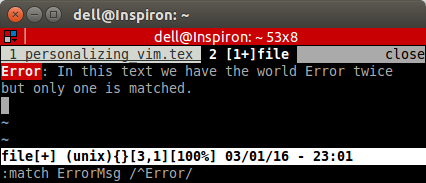
\includegraphics[scale=0.7]{./images/page23.png}
\end{center}

这个命令查找位于行的开始位置的单词 \newterm{Error} (带有脱字符 \texttt{\^}),
如果找到了一个匹配, 就把匹配的文本用色彩组 \texttt{ErrorMsg} 的颜色
标记起来 (通常是红底白字).

如果读者不太喜欢已有的色彩组, 也可以自己定义一个, 定义色彩组的命令是:
\begin{vimcmd}
:highlight MyGroup ctermbg=red guibg=red gctermfg=yellow
        guifg=yellow term=bold
\end{vimcmd}
这个命令创建了一个名为 \file{MyGroup} 的色彩组, 红底黄字, 在控制台 (Vim)
和 GUI (Gvim) 环境下都是如此. 用户可以根据自己的喜好, 修改下列选项:

\begin{center}
\begin{tabular}{ll}
    \hline
    \texttt{ctermbg}    & 控制台环境下的背景色 \\
    \texttt{guibg}      & Gvim 环境下的背景色 \\
    \texttt{ctermfg}     & 控制台环境下的文本颜色 \\
    \texttt{guifg}      & Gvim 环境下的文本颜色 \\
    \texttt{gui}        & Gvim 环境下的字体格式 \\
    \texttt{term}       & 控制台环境下的字体格式 (比如粗体: bold) \\
    \hline
\end{tabular}
\end{center}

如果使用了已有的色彩组的名字, 那么在接下来的会话中如果用到了该色彩组,
所使用的将会是修改后的效果.

使用匹配命令时, 给定的模式会一直匹配下去, 直到执行一个新的匹配, 或者执行
下列命令:
\begin{vimcmd}
:match NONE
\end{vimcmd}
\marginpar{24}
匹配命令一次只能匹配一个模式, 但是 Vim 另外提供了 2 个命令用于一次匹配至
多 3 个模式. 命令很容易记忆:
\begin{vimcmd}
:2match
:3match
\end{vimcmd}
读者也许想知道这些匹配命令应该在什么样的情况下使用, 因为在平时的话这些命令
没什么大用处. 这里有一些例子, 它们展示出了匹配的强大之处.

\subsection{示例 1: 用彩色标记某列后面的文字}
\label{subsec:mark_color_characters_after_a_certain}
在写邮件时, 一条比较常见的规则是一行的长度不能超过 74 个字符 (在某些古老
的编程语言中, 同样存在这样的规则). 在这种情况下, 当你在一行内写出的字符
数超过某个上限时, 如果 Vim 能够发出提醒那就再好不过了.

只需要下面这个命令就可以完成上面提到的功能:
\begin{vimcmd}
:match ErrorMsg /\%>73v.\+/
\end{vimcmd}
执行该命令后, 一行内的第 73 个字符之后的那些字符都会被标记成错误. 匹配命令 
中含有一个正则表达式, 这个表达式可以拆成:
\begin{center}
\begin{tabular}{ll}
    \hline
    \verb'\%>'  & 匹配该列之后的内容, 列号紧跟在尖括号的右边 \\
    \verb'73'   & 列号  \\
    \verb'v'    & 只能工作在可见的列上面 \\
    \verb'.\+'  & 匹配一个或多个任意的字符 \\
    \hline
\end{tabular}
\end{center}
\begin{center}
    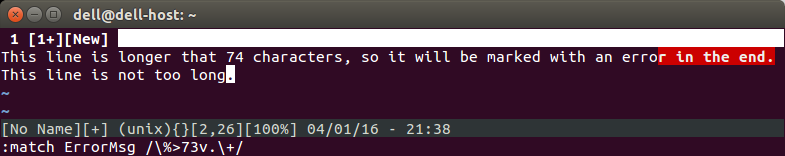
\includegraphics[scale=0.6]{./images/page24.png}
\end{center}
\marginpar{25}
\subsection{示例 2: 标记代码中未被用作缩进的制表符}
\label{subsec:mark_tabs_not_used_for_indentation_in_code}
编码时, 一条很重要的规则是制表符只被用作缩进代码, 其他地方则不允许使用制表
符. 然而, 对某些人来说常常会忘记该规则. 现在, 只需要一条简单的匹配命令, 就
可以时刻提醒着程序员.

下面这条命令把所有的, 不在行的开始位置上的制表符用错误信息的颜色标记出来:
\begin{vimcmd}
:match errorMsg /[^\t]\zs\t\+/
\end{vimcmd}
执行完该命令后, 你就可以看到是否违反了规则 --- 把制表符用在了代码内部. 把
命令分解开来看, 它由下列这几个部分组成:
\begin{center}
    \begin{tabular}{ll}
        \hline
        \verb'[^'   & 字符组的开始标记, 组中的字符将不会被匹配到 \\
        \verb'\t'   & 制表符 \\
        \verb']'    & 字符组的结束标记 \\
        \verb'\zs'  & 一个宽度为 0 的匹配, 它把 ``匹配'' 置于一行的开始,
        并忽略任意的空格 \\
        \verb'\t\+' & 匹配一个或多个制表符 \\
        \hline
    \end{tabular}
\end{center}

\begin{center}
    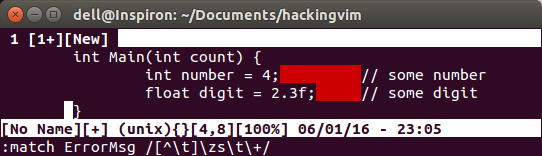
\includegraphics[scale=0.8]{./images/page25.png}
\end{center}

这个命令的意思是: 匹配所有的, 不在行的开始位置上的制表符 (忽略任意的空格).

如果你想用空格来缩进代码, 而不是制表符, 为了检查代码, 只需要把命令改成:
\begin{vimcmd}
:match errorMsg /[\t]/
\end{vimcmd}
这条命令的意思是: 匹配所有的制表符.
\marginpar{26}
\subsection{示例 3: 检查IP地址的有效性}
\label{subsec:preventing_errors_caused_by_ip_addresses}

如果用户需要在文本中写上大量的 IP 地址, 难免会出现错误 (例如
123.123.123.256). 为了防止出现这种情况, 可以把以下命令添加到文件
\file{vimrc} 中:
\begin{vimcmd}
match errorMsg /\(2[5][6-9]\|2[6-9][0-9]\|[3-9][0-9][0-9]\)[.]
               \[0-9]\{1,3\}[.][0-9]\{1,3\}[.][0-9]\{1,3\}\|
               \[0-9]\{1,3\}[.]\(2[5][6-9]\|2[6-9][0-9]\|\
                \\ \[3-9][0-9][0-9]\)[.][0-9]\{1,3\}[.][0-9]
                \\{1,3\}\|\[0-9]\{1,3\}[.][0-9]\{1,3\}[.]\(2[5]
                \\ \[6-9]\|\2[6-9][0-9]|[3-9][0-9][0-9]\)[.][0-9]\{1,3\}
             \\|[0-9]\{1,3\}[.][0-9]\{1,3\}[.][0-9]\{1,3\}[.]
             \\(2[5][6-9]\|2[6-9][0-9]\|\[3-9][0-9][0-9]\)/

\end{vimcmd}
相对于问题来说, 解决方法似乎有点太复杂了, 但请记住, 即使这条命令只能帮助你
一次, 但也值得把它加到配置文件.
\begin{warning}
从另一方面来看, 如果想匹配有效的 IP 地址, 只需要执行:
\begin{vimcmd}
    match todo /\(\(25[0-5]\|2[0-4][0-9]\|[01]\?[0-9]
                    [0-9]\?\)\.\)
                    \\ \{3\}\(25[0-5]\|2[0-4][0-9]\|[01]\?
                    [0-9][0-9]\?\)/
\end{vimcmd}
\end{warning}

\section{更丰富的状态行}
\label{sec:a_more_informative_status_line}
在 Vim 窗口的底部, 你会发现两样东西:
\begin{itemize}
    \item 命令行缓冲区 (输入命令的地方)
    \item 状态行
\end{itemize}
在默认的配置中, Vim 的状态行非常简单, 信息量也比较少. 状态行的右边显示
的是光标当前所在位置的行号与列号, 左边则是当前打开着的文件名 (如果有的话).

当执行 Vim 命令时, 状态行就会消失, 取而代之的是命令行缓冲区. 如果所执行的
命令带有输出信息, 那么这些信息就会出现在状态行的右侧.
\marginpar{27}
